\chapter{Introducción}

En el presente trabajo se realiza el análisis estadístico de texto, empleando como fuente a los comentarios de la transmisión en vivo del primer debate presidencial, realizado el día 7 de abril del 2024; los comentarios presentan una estructura lingüística mal estructurada, de igual forma, se identifican Emojis entre apalabras o comentarios completos a partir de los mismos.\\


\section{Primer objetivo}

\section{Segundo objetivo}


\chapter{descripción de los datos}



\begin{figure}[!h]
	\centering
	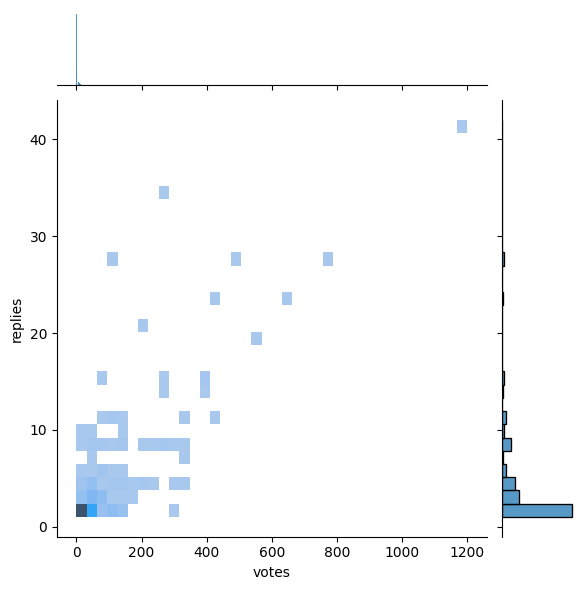
\includegraphics[width=13cm]{../Datos/AcumulacionYdistribuciones}
	\caption{grafico de frecuencias y distribución}
	\label{fig:FyD}
\end{figure}

\chapter{Procesado de los comentarios}





\chapter{Conclusiones}

